\documentclass[border=10pt]{standalone}

\usepackage{tikz}
\usepackage{tikzsymbols}
\usetikzlibrary{calc,patterns,shapes.geometric}

\def\centerarc[#1](#2)(#3:#4:#5){\draw[#1] ($(#2)+({#5*cos(#3)},{#5*sin(#3)})$) arc (#3:#4:#5);}

\begin{document}
	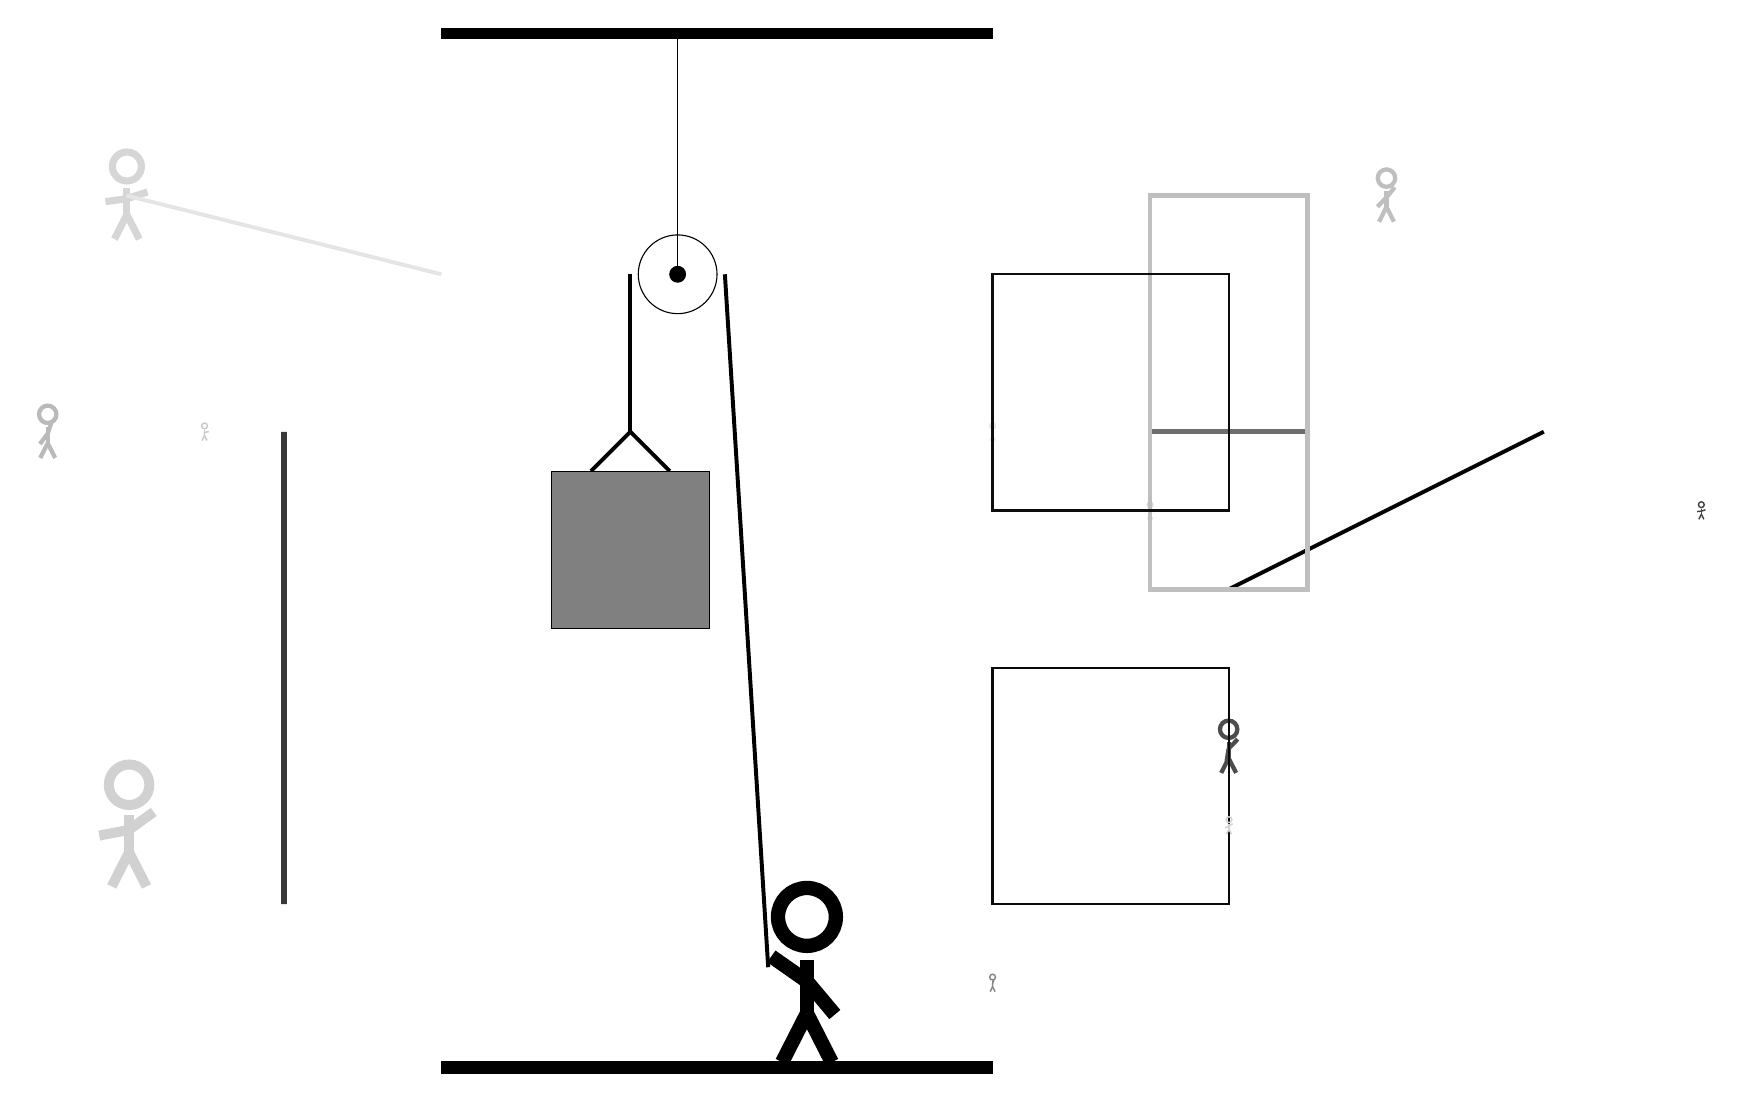
\begin{tikzpicture}
		%%%%% START %%%%%
		
		\draw[fill=black] (-2, 10) rectangle (5, 10.125);
		
		\node[line width=0.7mm, color=black!21] at (-5, 5) {\Strichmaxerl[1][87][10]};
		
		\node[line width=0.5mm, color=black!70] at (8, 1) {\Strichmaxerl[3][81][46]};
		\draw[line width=0.5mm, color=black!99](8, 3) -- (12, 5);
		\draw[line width=0.3mm, color=black!96] (5, -1) rectangle (8, 2);
		\node[line width=0.6mm, color=black!74] at (14, 4) {\Strichmaxerl[1][6][18]};
		\node[line width=0.6mm, color=black!48] at (5, -2) {\Strichmaxerl[1][88][71]};
		\draw[line width=0.7mm, color=black!78] (-4, 5) rectangle (-4, -1);
		\node[line width=0.2mm, color=black!14] at (7, 4) {\Strichmaxerl[1][89][73]};
		\node[line width=0.2mm, color=black!25] at (10, 8) {\Strichmaxerl[3][46][51]};
		\node[line width=0.7mm, color=black!10] at (5, 5) {\Strichmaxerl[1][78][87]};
		
		\node[line width=0.6mm, color=black!18] at (-6, 0) {\Strichmaxerl[7][11][36]};
		\draw[line width=0.6mm, color=black!57] (7, 3) rectangle (9, 5);
		\draw[line width=0.6mm, color=black!25] (7, 3) rectangle (9, 8);
		
		\node[line width=0.2mm, color=black!27] at (-7, 5) {\Strichmaxerl[3][53][72]};
		\node[line width=0.3mm, color=black!18] at (8, 0) {\Strichmaxerl[1][23][33]};
		\node[line width=0.6mm, color=black!16] at (-6, 8) {\Strichmaxerl[5][8][18]};
		
		\draw[line width=0.5mm, color=black!10](-2, 7) -- (-6, 8);
		\draw[line width=0.3mm, color=black!95] (5, 4) rectangle (8, 7);
		
		\draw (1, 7) circle (0.5);
		\draw[fill=black] (1, 7) circle (0.1);
		\draw (1, 10) -- (1, 7);
		
		\draw[line width=0.5mm] (-0.1, 4.5) -- (0.4, 5.0) -- (0.9, 4.5);
		\draw[fill=black!50] (-0.6, 4.5) rectangle (1.4, 2.5);
		
		\draw[line width=0.5mm] (0.4, 7) -- (0.4, 5.0);
		\centerarc[line width=0.5mm](1, 7)(0:180:0.6);
		\draw[line width=0.5mm](1.6, 7) -- (2.15, -1.8);
		
		\node at (2.6, -1.9) {\Strichmaxerl[10][-35][-50]};
		
		\draw[fill=black] (-2, -3) rectangle (5, -3.15);
		
		%%%%% END %%%%%
	\end{tikzpicture}
\end{document}